\section{System Overview}\label{sec:system-overview}
\subsection{Full Gesture Recognition System}\label{subsec:full-gesture-recognition-pipeline}
This research focuses on finding an appropriate neural network architecture to perform gesture recognition on a microcontroller, but it is only part of a larger project to create an entire gesture recognition system/pipeline.
The creation of this pipeline is composed of the following tasks:
\begin{enumerate}
    \item Optimizing the number and placement of OPT101 photo diodes.
    \item Pre-processing data from photo diodes.
    \item Creating an appropriate dataset for training a neural network to recognize gestures.
    \item Finding an appropriate neural network architecture on the created dataset and ensuring gestures can be recognized in real-time on an Arduino Nano 33 BLE\@.
\end{enumerate}

The research presented in this paper aims to complete task 4.
Although tasks 1--3 were completed by other project group members and are beyond the scope of this research, they are worth mentioning to provide some context regarding the rest of the gesture recognition system.
Due to the findings from these tasks, the final system uses 3 photodiodes and can recognize 10 different gestures, while each gesture is composed of 100 time steps from each photodiode.
This is relevant for task 4, as it means that whatever neural network is implemented must use a 2D array of size 3 by 100 (split into \textit{n} frames after 3D-formatting) as an input feature and be able to distinguish between 10 output classes, as illustrated in figure~\ref{fig:system}.

\begin{figure}[h]
    \centering
    \captionsetup{justification=centering}
    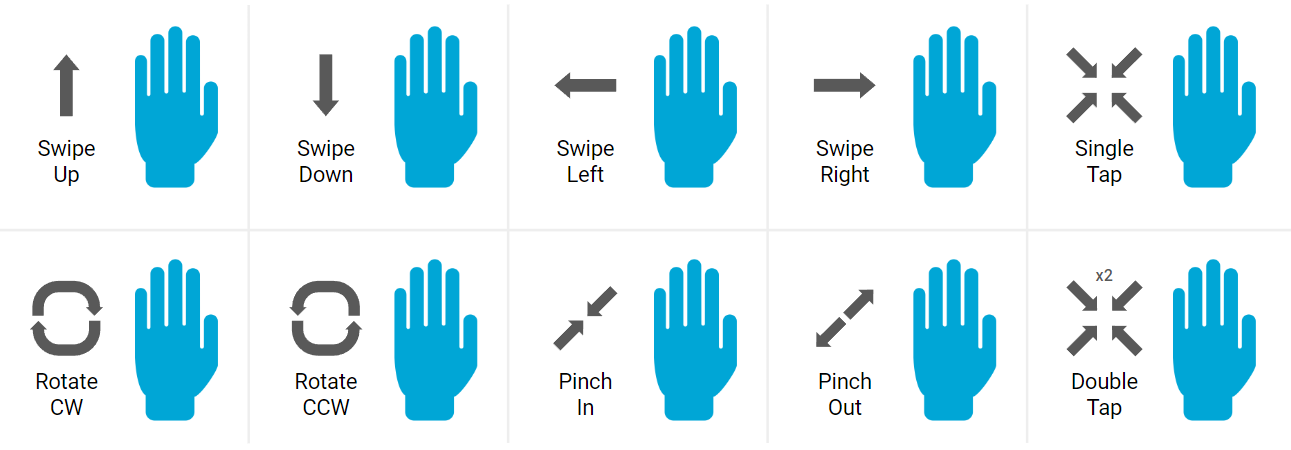
\includegraphics[width=\linewidth]{figures/gestures}
    \caption{Illustrations of the 10 different gestures that the system can recognize.}
    \label{fig:gestures}
\end{figure}

\begin{figure}[h]
    \centering
    \captionsetup{justification=centering}
    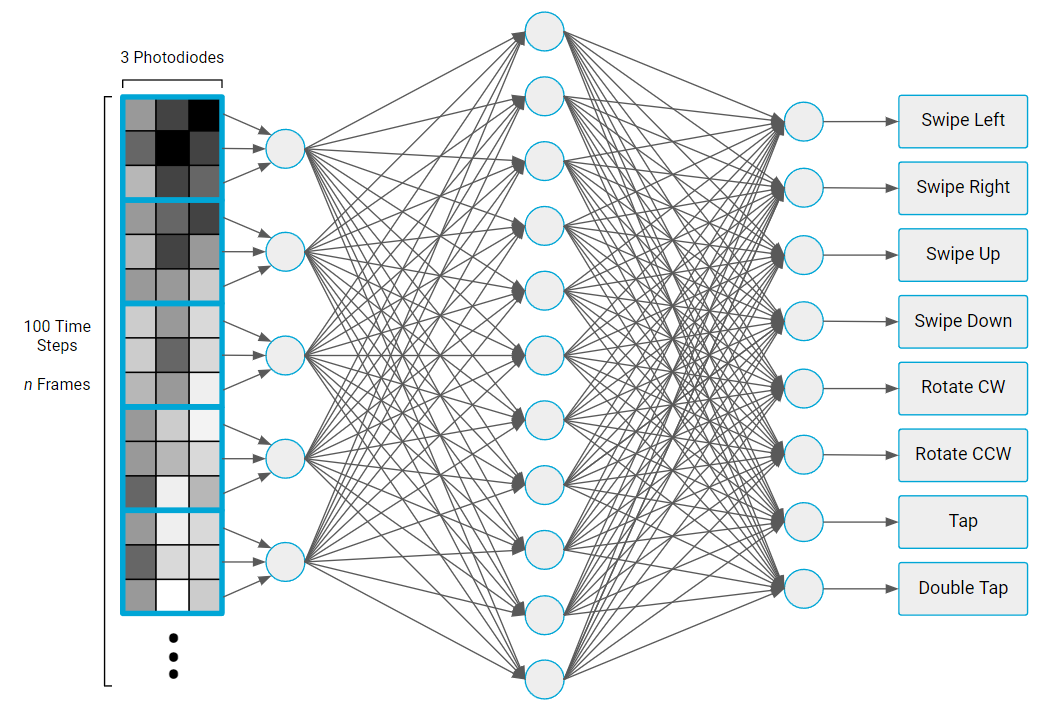
\includegraphics[width=\linewidth]{figures/system_advanced}
    \caption{Visualization of the input features \& output classes using a generic artificial neural network as an example.}
    \label{fig:system}
\end{figure}

\subsection{System Caveats}\label{subsec:system-caveats}
The overarching goal of the project that this research contributes to is the creation of a full gesture recognition pipeline, which presents some issues when considering the fact that each part of this pipeline was developed in parallel due to the limited time allotted for the project.
In reality, it would make much more sense to complete each step of the pipeline sequentially, as the performance of later parts of the pipeline relies on the performance of previous parts.
To put this in the context of the gesture recognition system, it is impossible to train a neural network to recognize gestures without first having a dataset to train it on.
However, the creation of that dataset relies on photodiode count and placement, as well as sampling rate and pre-processing, being finalized.
If they change after the dataset is completed, it will not be representative of real-world data, leading to poor gesture classification performance from the neural network trained on it.

\subsection{Dataset}\label{subsec:dataset}
Having a varied, expansive, and representative dataset is crucial for training a machine learning with high real-world accuracy.
Fortunately, a dataset for recognizing gestures using photodiode data was done by another member of the project group, as mentioned in section~\ref{subsec:full-gesture-recognition-pipeline}.

Unfortunately, because the allotted time for the project meant that all group members had to work in parallel, as stated in section~\ref{subsec:system-caveats}, the neural networks evaluated in this paper had to be trained on a dataset that is not final.
Specifically, the dataset used in this research is not passed through the data pre-processing stage of the system.
This means that the neural networks presented in this paper were trained on raw data from the photodiodes, whereas real-world data on the final system would include this pre-processing step.
This leads to model accuracy being lower than it could be, as there is noise and other artifacts in the raw photodiode data.

The dataset used contains 5 repetitions of each of the 10 gestures per hand across 48 participants/candidates, leading to 4800 total data instances.
Each instance is made up of a 5 second window during which a gesture is performed over the photodiodes, with a sampling rate of 20Hz for candidates 1--27 and 100Hz for candidates 28--48, for of 100 samples per photodiode and 500 samples per photodiode respectively.
However, the instances recorded at 100Hz are down-sampled back to 20Hz so that the data format remains consistent across the whole dataset.

Although the dataset contains instances from a variety of environments and lighting setups, these are mostly indoor locations as this is the planned use case for the system.
The dataset was also mostly recorded on the TU Delft campus, meaning the demographic of participants is somewhat skewed.
Most notably, the dataset contains substantially more instances of males compared to females, and more right-handed participants than left-handed.
However, this is not expected to have a large impact on the performance on any neural networks trained on this dataset.